\documentclass[11pt]{article}

\usepackage{natbib,rotfloat,epsfig,setspace,amssymb,amsmath, comment}

\setlength{\hoffset}{0.2in}
\setlength{\voffset}{-0.6in}
\setlength{\textwidth}{6.0in}
\setlength{\evensidemargin}{0in}
\setlength{\oddsidemargin}{0in}
\setlength{\textheight}{8.5in}

\begin{document}

\onehalfspace

\title{Economics 512 -- Homework 6}
\author{Due January 21, 2019}
\date{}
\maketitle
This assignment extends Problem 7.4 in in Miranda \& Fackler. 
Consider competitive price-taking firm that maximizes discounted sum of expected future profits from harvesting a non-renewable resource. 
For example, suppose a lumber company is deciding how many trees to harvest in a forest where trees do not grow back. 
The discount factor of our lumber company is $\delta = 0.95$. The firm earns revenue of $p\cdot x$ per period if it has harvested amount $x$ and market price was $p$. To harvest $x$ the firm incurs a convex cost $0.2\cdot x^{1.5}$. The firm is small relative to the market, and has rational expectations that the price of lumber
will follow an AR(1) process: 
\begin{align}
p_t = p_0 + \rho\cdot p_{t-1} + u
\end{align}
Where $p_0 = 0.5$, $\rho = 0.5$, and $u$ is a mean-zero normal disturbance with standard deviation $\sigma_u=0.1$.
The initial stock of lumber may be anything from 0 to 100.
%\footnote{Note that there is non-zero unconditional probability of price being negative, however it is very unlikely, so we will ignore it.} 
\begin{enumerate}
\item Formulate firm's dynamic optimization problem. Specifically, formulate the Bellman equation, identify state and policy variables, their spaces and transition probabilities. Assume initial stock is between 0 and 100.\\[1em]
Let the initial stock be $s_0$. Then the Bellman equation is:
$$ 
V(s,p)= \max_{s' \in [0,s]} \{p(s-s')- 0.2*(s-s')^{1.5}+\delta  \mathbb{E}[V(s', p')|p]\}
$$
The state variables are $(s,p)$, the current stock and current market price. Policy variable is $s'$, the stock to hold for next period. The state space is $[0,s_0]\times [0, \infty]$. The policy space is $[0,s]$. The market price follows an AR(1) process, so the transition probability to any point state is zero. However, we can approximate the AR(1) process with a Markov process in question 2. 


\item Take a look at {\tt tauchen.m} in the repository (you should know where), use it to generate grid that approximates process for $p_t$ with 21 grid points. \\[1em]

It's done in the programming.

\item Solve the firm's problem using value function iteration. Plot the value of the firm depending on its initial stock (x-axis) and the current price of lumber, for $p \in{0.9, 1, 1.1}$.\\[1em]

I solved the dynamic programming problem using the value function iteration. The relationship between firm value and initial stock when holding current price of lumber fixed is plotted as followed: \\
    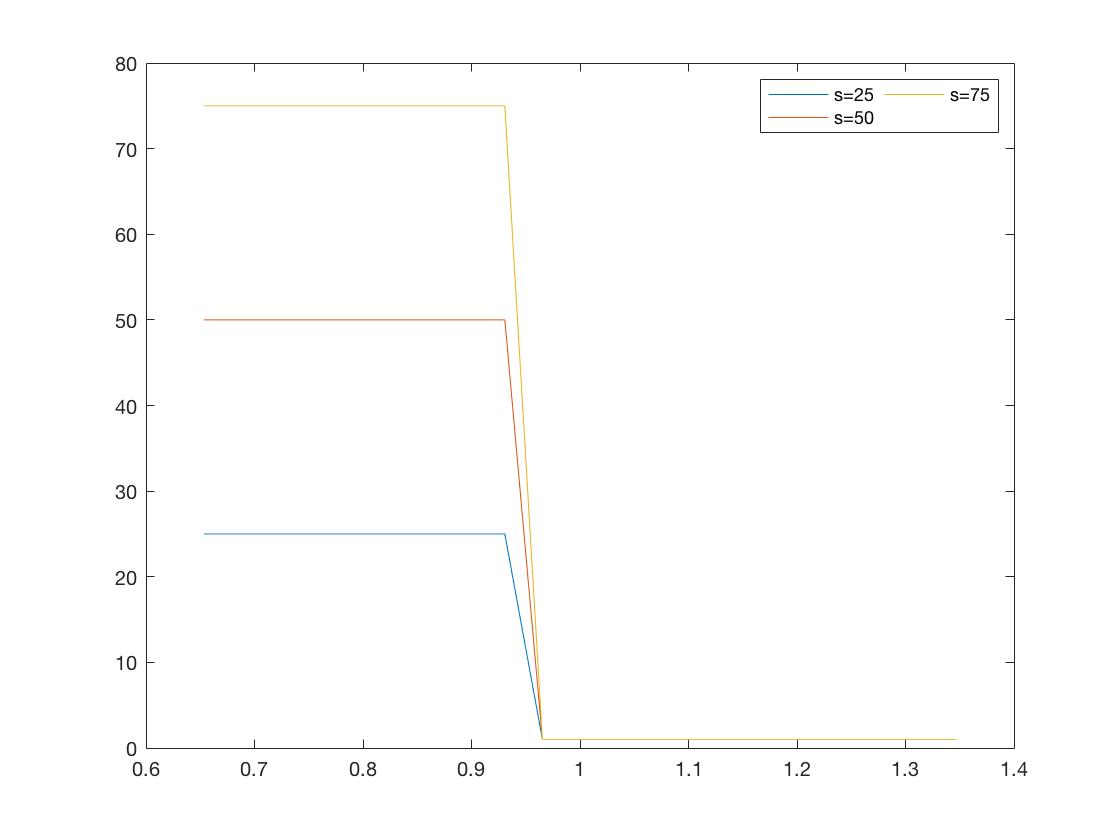
\includegraphics[scale=0.2]{Vs0.jpg}


\item Plot next period optimal stock (or harvest amount if you prefer) as a function of today's price for different amount of lumber left in stock.\\[1em]

The relationship between next period optimal stock and the price when holding amount of lumber left in stock as 25, 50 or 75 are plotted as:\\
    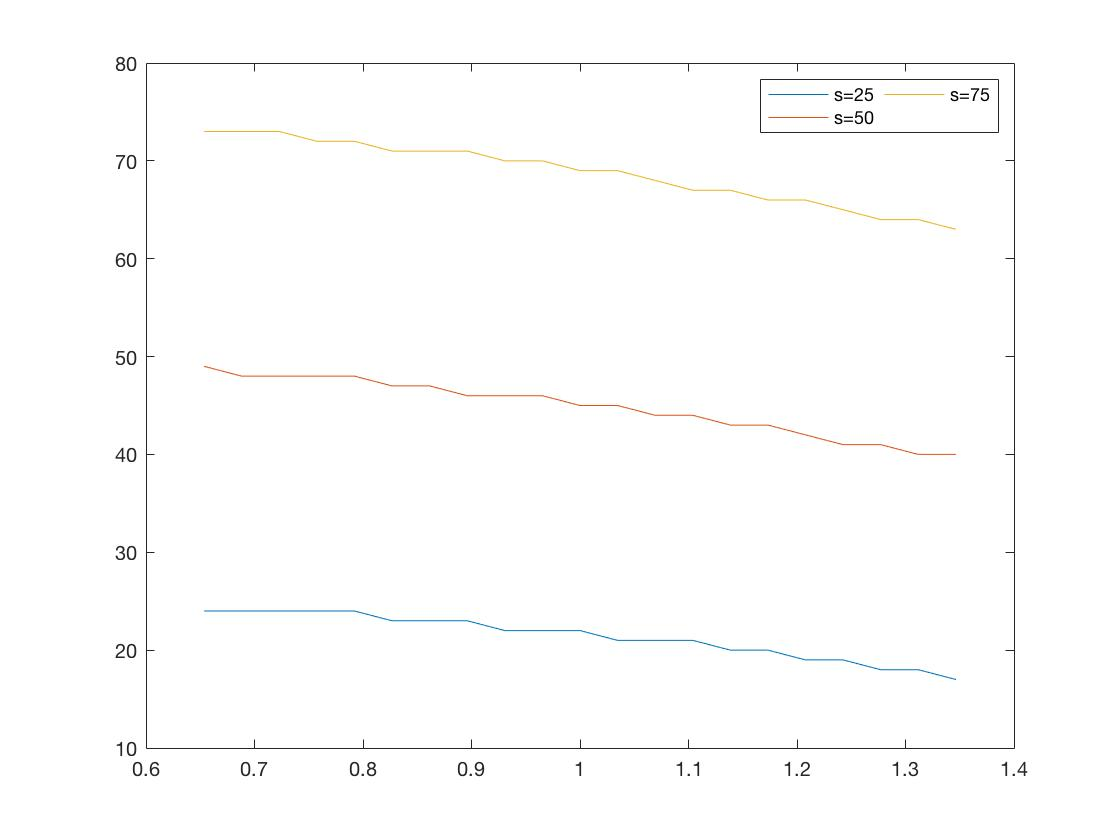
\includegraphics[scale=0.2]{spolp.jpg}


\item Assume firm starts with stock of 100 and today's price is 1. Plot expected stock over time for 20 periods ahead. Include the 90 percent confidence interval. \\[1em]

The expected stock decreases over time from 93 to about 10. The evolution process is illustrated as: \\
 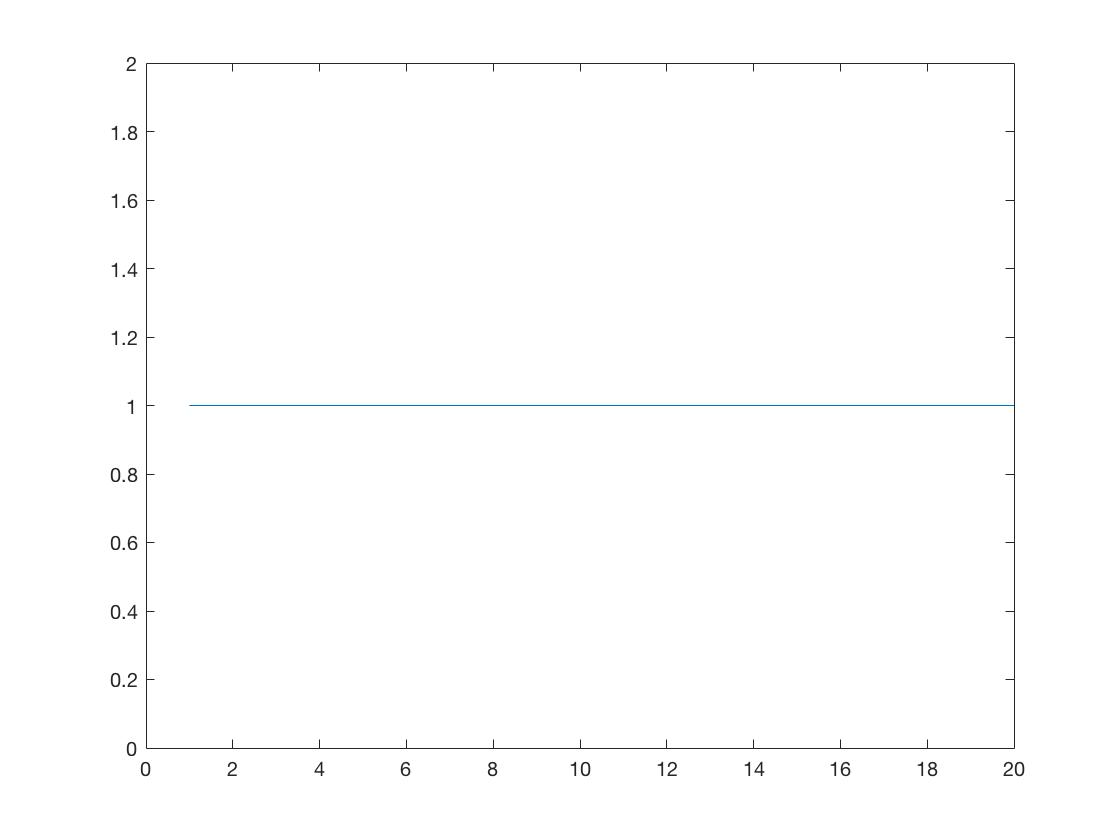
\includegraphics[scale=0.2]{spath.jpg}

\item Redo the 2-4 for coarse grid of 5 points in Tauchen's representation.\\[1em]

I solved the dynamic programming problem using the value function iteration. The relationship between firm value and initial stock when holding current price of lumber fixed is plotted as followed: \\
    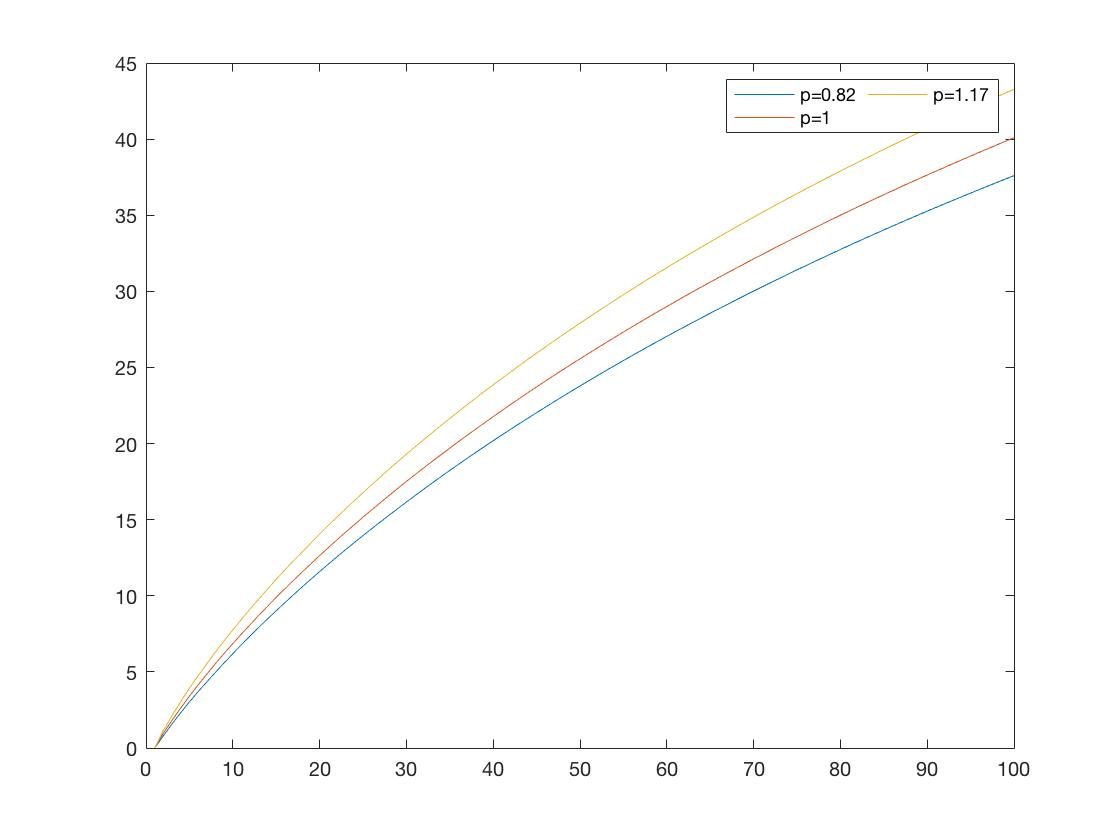
\includegraphics[scale=0.2]{Vs0_5.jpg} \\
The relationship between next period optimal stock and the price when holding amount of lumber left in stock as 25, 50 or 75 are plotted as:\\
    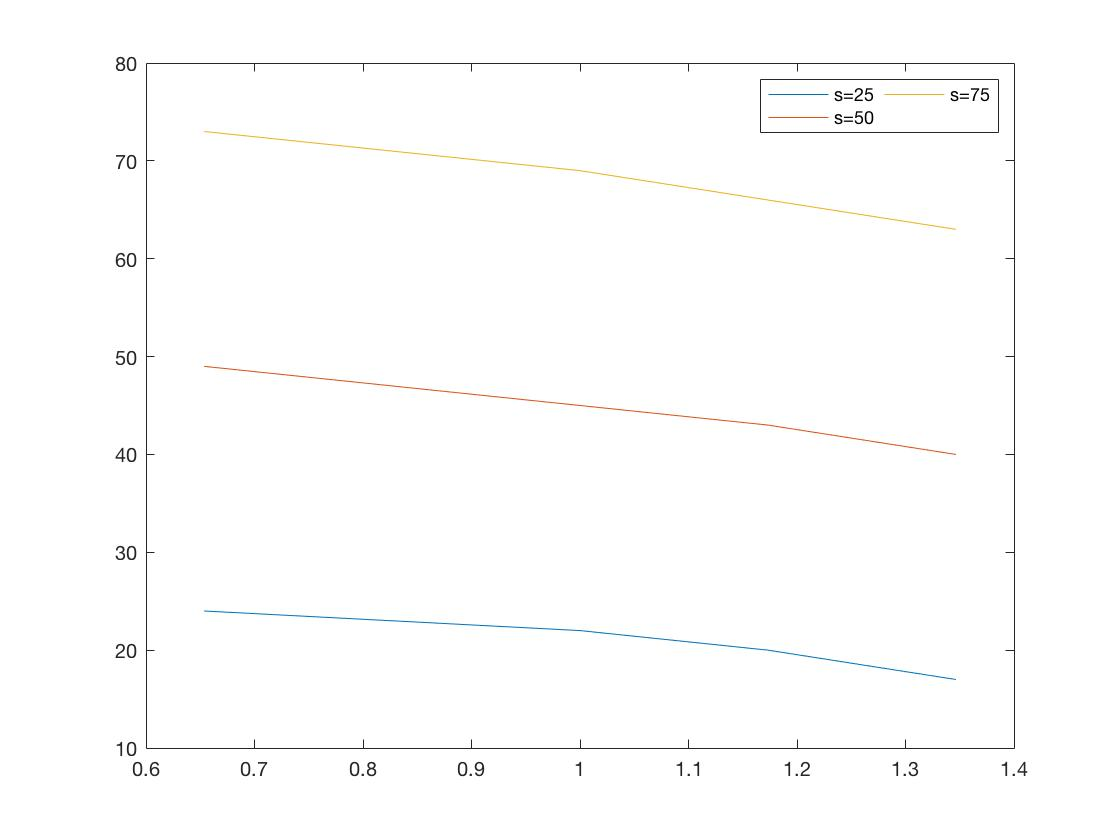
\includegraphics[scale=0.2]{sp_5.jpg}

\item Submit your code together with a pdf of your responses in \LaTeX. (Yes, part of this assignment is to get you to embed figures into \LaTeX.)
\end{enumerate}


\end{document}
